\section{Fatores Externos}

\subsection {Altitude}

\begin{figure}[h!]
\centering
{\scriptsize Tabela 5: Estatísticas de tendência central e dispersão para a altitude (m) da sede dos municípios em cada banco de dados: WAV = Wikiaves, SLI = SpeciesLink. n = número de municípios, m = média, dp = desvio-padrão, min-max = valores extremos, q1-q3 = quartis. Foram excluídos dessa análise os municípios com altitude inferior a 250 m e superior a 1200 m.}
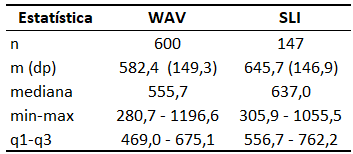
\includegraphics{Tabelas/5.png}
\end{figure}

\texto

\begin{figure}[h!]
\centering
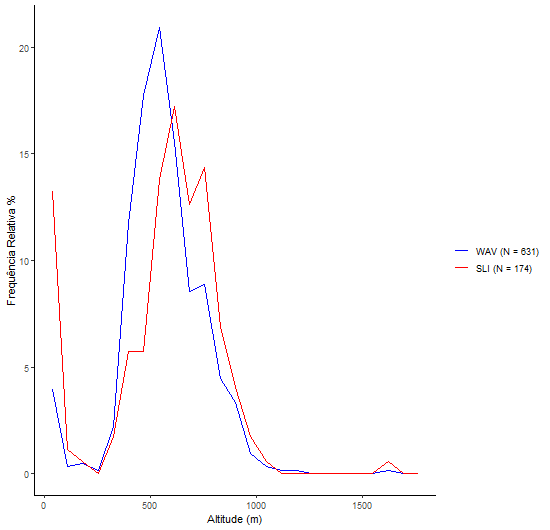
\includegraphics[height = 8cm]{Imagens/213.png}
\\{\scriptsize Figura 4: Distribuição de municípios em classes segundo a altitude (m) de sua sede em cada banco de dados: WAV = Wikiaves, SLI = SpeciesLink. n = número de municípios. Foram excluídos da análise da Tabela 5 os municípios com altitude inferior a 250 m e superior a 1200 m.}
\end{figure}

\newpage

\subsection{Área}

\begin{figure}[h!]
\centering
{\scriptsize Tabela 6: Estatísticas de tendência central e dispersão para a área (Log10 km2) dos municípios em cada banco de dados: WAV = Wikiaves, SLI = SpeciesLink. n = número de municípios, m = média, dp = desvio-padrão, min-max = valores extremos, q1-q3 = quartis. Foram excluídos dessa análise os municípios com área inferior a X km2.}
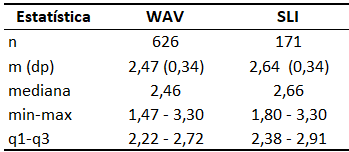
\includegraphics{Tabelas/6.png}
\end{figure}

\texto



\begin{figure}[h!]
\centering
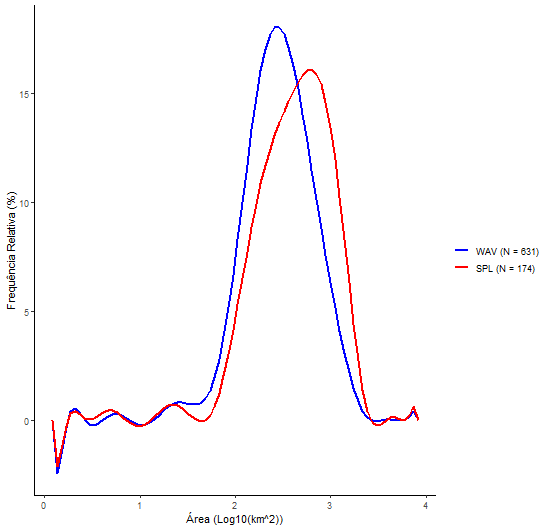
\includegraphics[height = 8cm]{Imagens/223.png}
\\{\scriptsize Figura 5: Distribuição de municípios em classes segundo a área (Log10 km2) em cada banco de dados: WAV = Wikiaves, SLI = SpeciesLink. n = número de municípios. Foram excluídos da análise da Tabela 6 os municípios com área inferior a X km2.}
\end{figure}

\newpage

\subsection{População}

\begin{figure}[h!]
\centering
{\scriptsize Tabela 7: Estatísticas de tendência central e dispersão para o tamanho da população humana (Log10 indivíduos) dos municípios em cada banco de dados: WAV = Wikiaves, SLI = SpeciesLink. n = número de municípios, m = média, dp = desvio-padrão, min-max = valores extremos, q1-q3 = quartis. Foi excluído dessa análise o município com 12252023 habitantes (São Paulo).}
\\
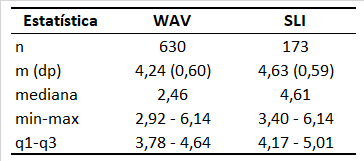
\includegraphics{Tabelas/7.png}
\end{figure}

\texto

\begin{figure}[h!]
\centering
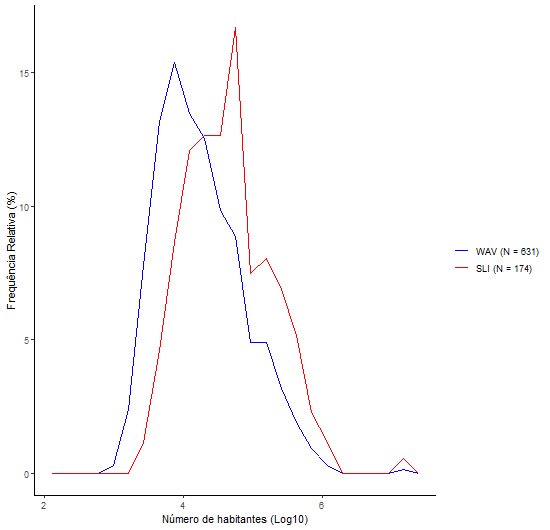
\includegraphics[height = 8cm]{Imagens/233.png}
\\{\scriptsize Figura 6: Distribuição de municípios em classes segundo o tamanho da população humana (Log10 indivíduos) em cada banco de dados: WAV = Wikiaves, SLI = SpeciesLink. n = número de municípios. Foi excluído da análise da Tabela 7 o município com 12252023 habitantes (São Paulo).}
\end{figure}

\newpage

\subsection{Latitude}

\begin{figure}[h!]
\centering
{\scriptsize Tabela 8: Estatísticas de tendência central e dispersão para a latitude (graus) da sede dos municípios em cada banco de dados: WAV = Wikiaves, SLI = SpeciesLink. n = número de municípios, m = média, dp = desvio-padrão, min-max = valores extremos, q1-q3 = quartis.}
\\
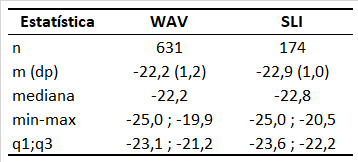
\includegraphics{Tabelas/8.png}
\end{figure}

\texto

\begin{figure}[h!]
\centering
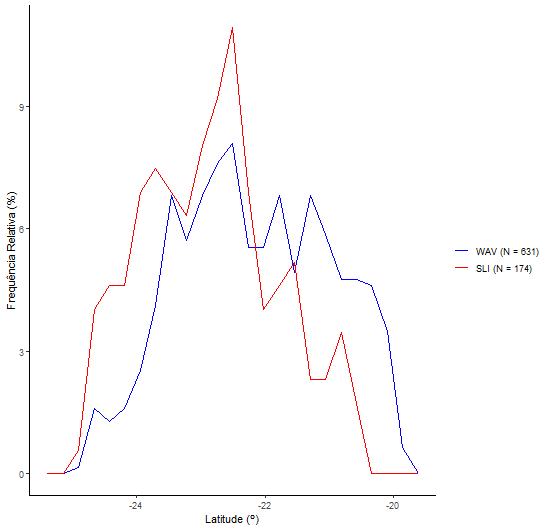
\includegraphics[height = 8cm]{Imagens/243.png}
\\{\scriptsize Figura 7: Distribuição de municípios em classes a latitude (graus) da sede dos municípios em cada banco de dados: WAV = Wikiaves, SLI = SpeciesLink. n = número de municípios.}
\end{figure}

\newpage

\subsection{Longitude}


\begin{figure}[h!]
\centering
{\scriptsize Tabela 9: Estatísticas de tendência central e dispersão para a longitude (graus) da sede dos municípios em cada banco de dados: WAV = Wikiaves, SLI = SpeciesLink. n = número de municípios, m = média, dp = desvio-padrão, min-max = valores extremos, q1-q3 = quartis.}
\\
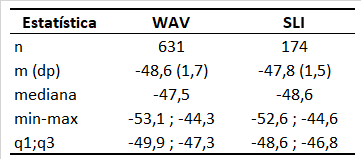
\includegraphics{Tabelas/9.png}
\end{figure}

\texto


\begin{figure}[h!]
\centering
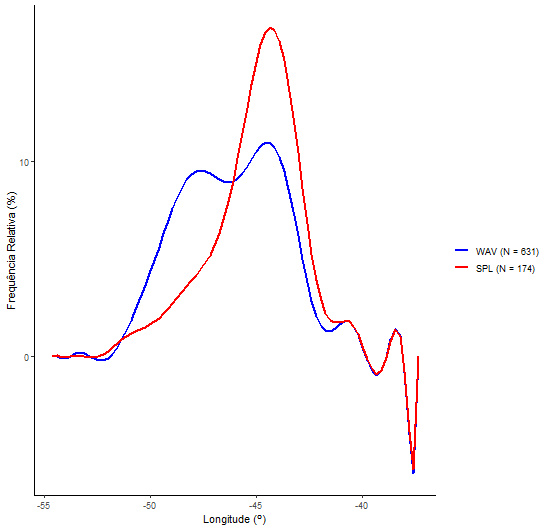
\includegraphics[height = 8cm]{Imagens/253.png}
\\{\scriptsize Figura 8: Distribuição de municípios em classes a longitude (graus) da sede dos municípios em cada banco de dados: WAV = Wikiaves, SLI = SpeciesLink. n = número de municípios.}
\end{figure}

\newpage
